% STEP 1: Choose oneside or twoside. Use the 'draft' option a lot when writing.
\documentclass[english, oneside]{HYgradu}

\usepackage[utf8]{inputenc} % For UTF8 support. Use UTF8 when saving your file.
\usepackage{lmodern} % Font package
\usepackage{textcomp}
\usepackage[pdftex]{color, graphicx} % For pdf output and jpg/png graphics
\usepackage[pdftex, plainpages=false]{hyperref} % For hyperlinks and pdf metadata
\usepackage{fancyhdr} % For nicer page headers
%\usepackage{tikz} % For making vector graphics (hard to learn but powerful)
%\usepackage{wrapfig} % For nice text-wrapping figures (use at own discretion)
\usepackage{amsmath, amssymb} % For better math
\usepackage[round]{natbib} % For bibliography
\usepackage[footnotesize,bf]{caption} % For more control over figure captions
\usepackage{subcaption}

\fussy % Probably not needed but you never know...


% OPTIONAL STEP: Set up properties and metadata for the pdf file that pdfLaTeX makes.
% But you don't really need to do this unless you want to.
\hypersetup{
    bookmarks=true,         % show bookmarks bar first?
    unicode=true,           % to show non-Latin characters in Acrobat’s bookmarks
    pdftoolbar=true,        % show Acrobat’s toolbar?
    pdfmenubar=true,        % show Acrobat’s menu?
    pdffitwindow=false,     % window fit to page when opened
    pdfstartview={FitH},    % fits the width of the page to the window
    pdftitle={},            % title
    pdfauthor={},           % author
    pdfsubject={},          % subject of the document
    pdfcreator={},          % creator of the document
    pdfproducer={pdfLaTeX}, % producer of the document
    pdfkeywords={something} {something else}, % list of keywords for
    pdfnewwindow=true,      % links in new window
    colorlinks=true,        % false: boxed links; true: colored links
    linkcolor=black,        % color of internal links
    citecolor=black,        % color of links to bibliography
    filecolor=magenta,      % color of file links
    urlcolor=cyan           % color of external links
}

% STEP 2:
% Set up all the information for the title page and the abstract form.
% Replace parameters with your information.
\title{Formation of cores by merging supermassive black holes}
\author{Joonas Suortti}
\date{\today}
\level{Master's thesis}
\faculty{Faculty of Whatever}
\department{Department of Something}
\address{PL 42 (Kuvitteellinen katu 1)\\00014 Helsingin yliopisto}
\subject{Your Field}
\prof{prof. Smith}
\censors{prof. Smith}{doc. Smythe}{}
\depositeplace{}
\additionalinformation{}
\numberofpagesinformation{\numberofpages\ pages}
\classification{}
\keywords{Your keywords here}
\quoting{``Bachelor's degrees make pretty good placemats if you get them laminated.'' \\---Jeph Jacques}

\begin{document}

% Generate title page.
\maketitle

% STEP 3:
% Write your abstract (of course you really do this last).
% You can make several abstract pages (if you want it in different languages),
% but you should also then redefine some of the above parameters in the proper
% language as well, in between the abstract definitions.
\begin{abstract}
Abstract goes here.
\end{abstract}

% Place ToC
\mytableofcontents



% -----------------------------------------------------------------------------------
% STEP 4: Write the thesis.
% Your actual text starts here. You shouldn't mess with the code above the line except
% to change the parameters. Removing the abstract and ToC commands will mess up stuff.
\chapter{Introduction}

\chapter{Theory}

\chapter{KETJU}

\chapter{KETJU Results}

We analyse the results from two sets of early type galaxy merger KETJU simulations, where the progenitor galaxies contain supermassive black holes, with masses ranging from $8.5 \times 10^8 M_\odot$ to $8.5 \times 10^9 M_\odot$, in their centre \citep{Mannerkoski2019, Rantala2018}. 

\section{Simulation Details}

Both simulation sets use the same progenitor galaxies in their simulations.

The results from the simulations done by \cite{Mannerkoski2019} contain only the locations, velocities and the masses of the central black holes of the progenitor galaxies at different time steps; starting from the step where the semi-major-axis of the SMBH system is $a \lesssim 5000 R_s$, where $R_s$ is the Schwarzschild radius, up until the end of the simulation. We will show the initial conditions in more detail in the next subsection.

The simulation results of \cite{Rantala2018} consist of the properties of not only the black holes, but also the stellar particles and dark matter particles. This data comes from a single time before the merging of the black holes step at $t = 2 \mathrm{Gyr}$ of in the simulation time. Once again, we will describe the initial conditions of the specific simulations in more depth later.

To make the päppäpäppä distinction between the different type of simulation results clearer, we will be calling the results from \cite{Mannerkoski2019} "runs", as they contain data from multiple simulation time steps; and the single time step results by \cite{Rantala2018} "snapshots".


\section{Black Hole Trajectories}

\begin{figure}[h]
	\centering	
	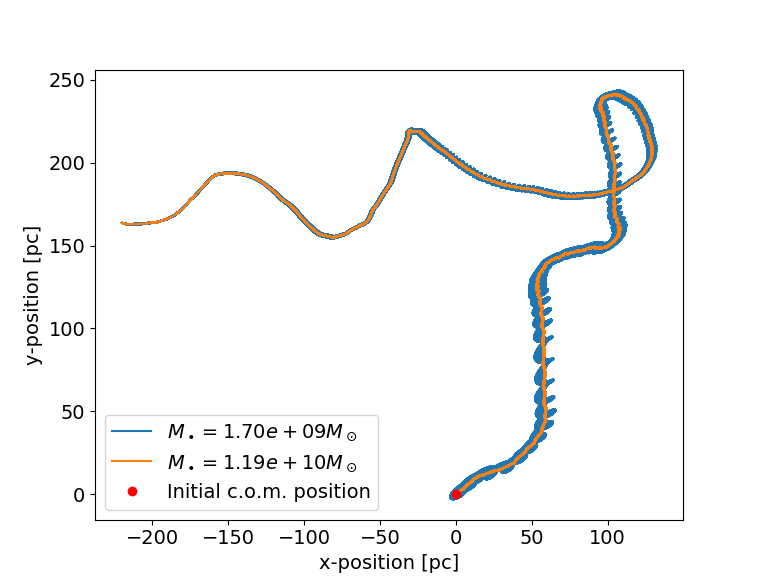
\includegraphics[width=0.7\textwidth]{Run3_Trajectory.png}	
	\caption{The trajectories of the black holes during "run 3" of the simulation. The coordinates are centred on the initial location of the centre-of-mass of the black hole system. The orange and blue lines show the paths taken by the smaller and larger black holes respectively during the simulation. Both paths show clear spiral patterns which become smaller and smaller as the simulation proceeds. The paths end at the location where the black holes merge, i.e. where the distance between them is below the specific threshold.}
\end{figure}

\begin{figure}[h]
	\centering
	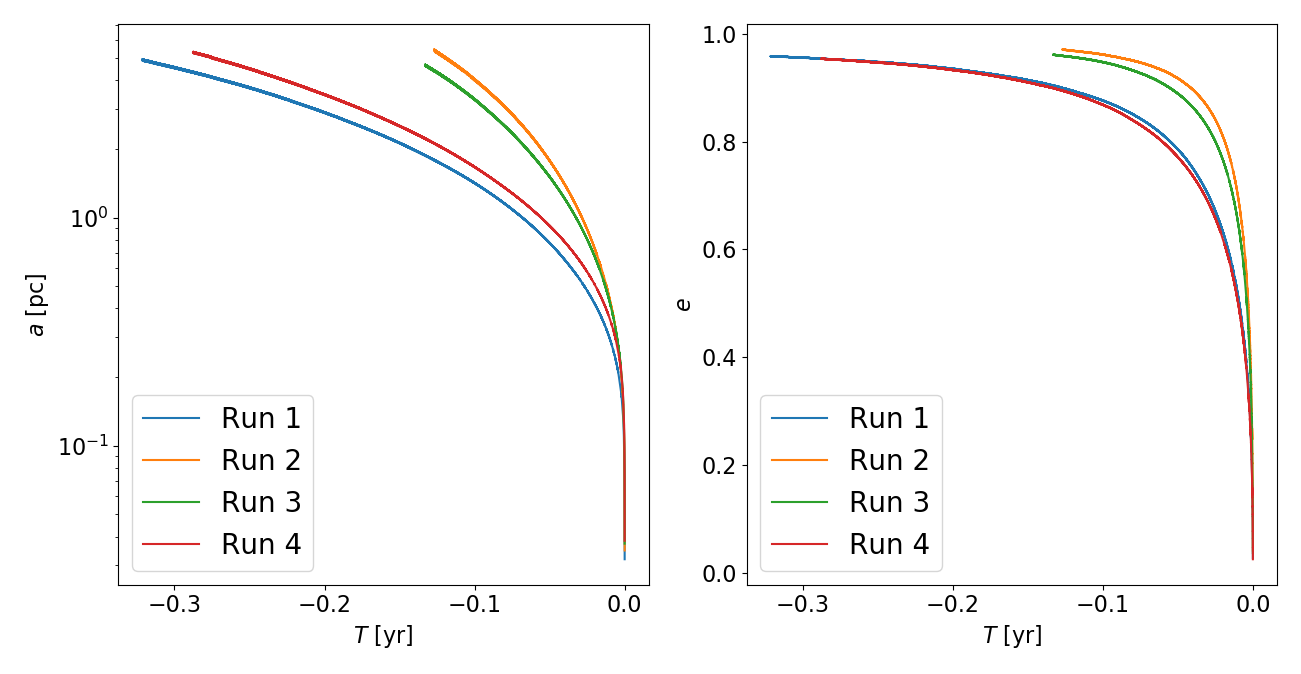
\includegraphics[width=\textwidth]{semi_major_and_ecc.png}
	\caption{The semi-major axes (left) and eccentricities (right) of the black hole systems in simulation runs 1-4 as a function of time. The zero position on the x-axis corresponds to the point of time in the simulation, where the black hole merging event happens.}
\end{figure}

\section{Core Radius Measurements}

Since the core of a cored galaxy is defined as a deviation from the expected theoretical surface brightness profile, determining its size requires us to: not only calculate surface brightness profiles from the simulation results, but also try to model the results with theoretical models that somehow take the brightness deficiency of the core region into account, as the starting location of the deviations from the expected can't be measured by eye.

We calculate the surface brightness profiles from the simulation snapshots by \cite{Rantala2018} by: projecting the stellar particles onto a plane and calculating the mass inside logarithmically space radial bins. In order to get a smooth density profile, we do this 100 times from random viewing angles and calculate the azimuthal averages of the binned masses. This allows us to form a mass surface density profile, which we then turn into a surface brightness profile by assuming a mass-to-light ratio of $M/L = 4$. In figure \ref{figure:surface_brightness}, one can see example surface brightness profiles for all of the simulated merger remnants. As can already be seen from the figure, the higher the mass of the central black holes in the progenitor galaxies, the larger the surface brightness deficiency near the center.

\begin{figure}[h]
	\centering
	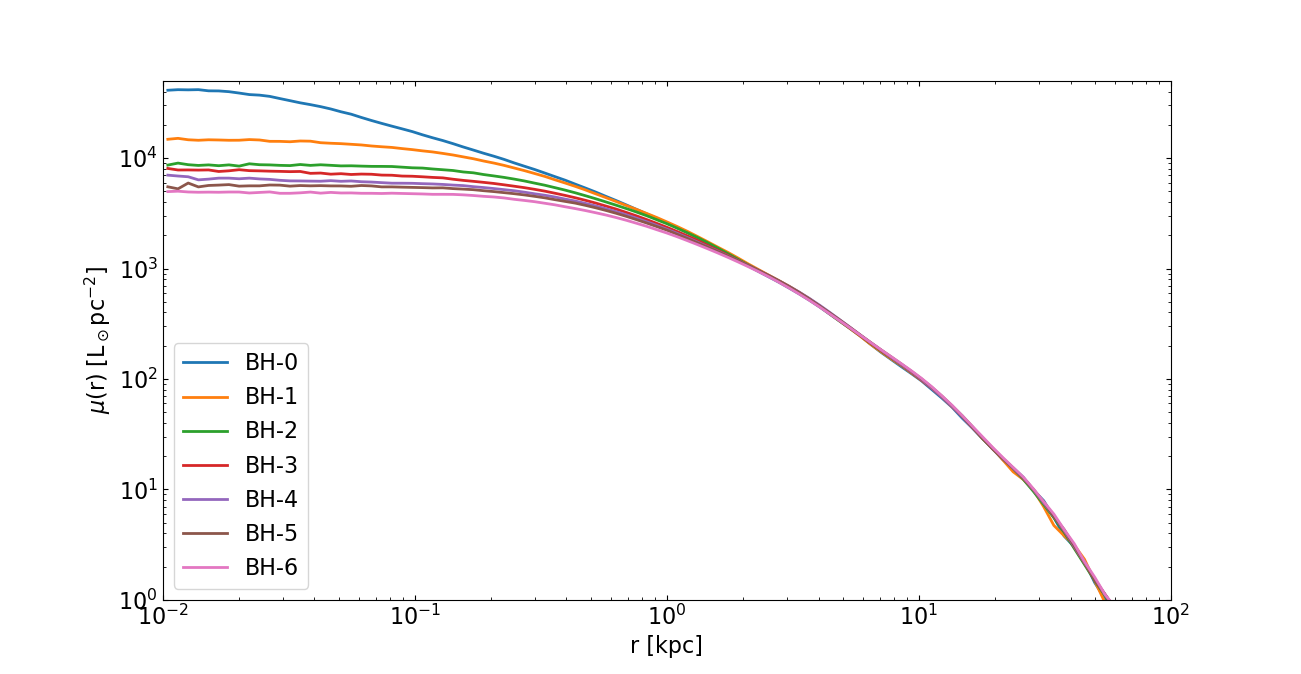
\includegraphics[width=\textwidth]{SurfaceBrightnessProfiles.png}
	\caption{Surface brightness profiles of all of the simulated merger remnants. The profiles were calculated by dividing the remnants into 100 radial bins, and averaging the surface brightness inside the bins through 100 random viewing angles. The luminosity of the particles was estimated by assuming a mass-to-light ratio of $M/L = 4$.}
	\label{figure:surface_brightness}
\end{figure}

As stated before, in order to calculate the sizes of the cores from profiles such as the ones seen in figure \ref{figure:surface_brightness}, we need to fit some kind of theoretical model that can describe a profile with surface brightness deficiency near the galactic centre onto the measured quantity. There are two commonly used options of profiles used for measuring the core size. The first one is the core-Sérsic profile \citep{Graham2003}:
\begin{equation}
\mu(r) = \mu' \left[ 1 + \left( \frac{r_b}{r} \right)^\alpha \right]^{\gamma / \alpha} \exp \left\lbrace -b_n \left[ \left( r^\alpha + r_b^\alpha \right) / r_e^\alpha \right]^{1/(\alpha n)} \right\rbrace, \label{eq:core-sersic}
\end{equation}
which divides the single power law Sérsic profile into a combination of an inner and outer power-law, and where $r_b$ is the break radius (i.e. the core radius), $\gamma$ is the logarithmic slope of the inner power-law, $\alpha$ controls the sharpness of the transition between the two power-laws, $r_e$ and $n$ are the effective half-mass radius and the Sérsic index of the outer power-law, and $\mu'$ is defined by:
\begin{equation}
\mu' = \mu_b 2^{-\gamma/\alpha} \exp \left[ b_n \left( 2^(1/\alpha) r_b/r_e \right)^{1/n} \right], 
\label{eq:mu_dot}
\end{equation}
where $\mu_b$ is the surface brightness at the break radius. 

The second option for calculating the core radius is the so called Nuker profile \citep{Lauer1995}:
\begin{equation}
\mu(r) = 2^{(\beta - \gamma) / \alpha} \mu_b \left( \frac{r_b}{r} \right)^\gamma \left[ 1 + \left( \frac{r}{r_b} \right)^\alpha \right]^{(\gamma - \beta)/\alpha},
\label{eq:nuker}
\end{equation}
where $r_b$ is once again the break radius (core radius), $\mu_b$ is the surface brightness at the core radius, $\beta$ and $\gamma$ are the logarithmic slopes of the power-laws inside and outside of the break radius respectively, and $\alpha$ is the sharpness of the transition between the two slopes.

\begin{figure}[h]
	\centering
	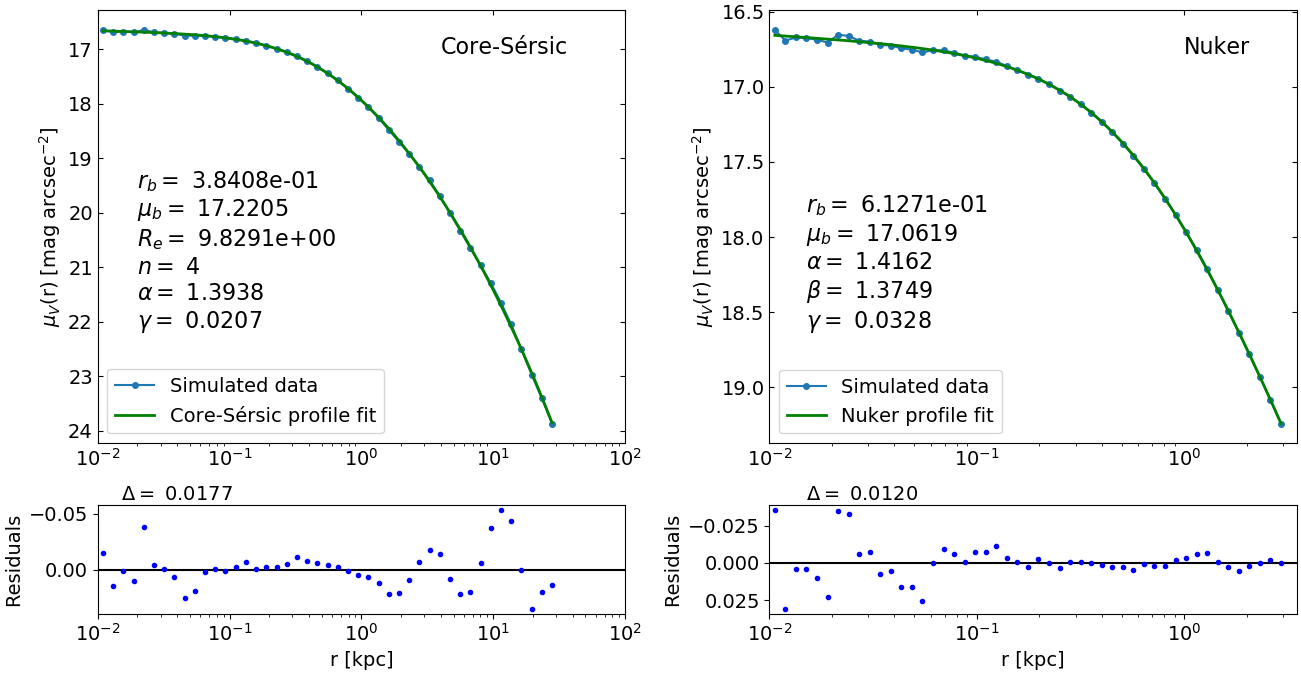
\includegraphics[width=\textwidth]{core_nuker_fits.png}
	\caption{Core-Sérsic and Nuker profile fits of surface brightness profiles calculated from the result of a merger simulation with progenitors containing $3.4 \times 10^9 M_\odot$ mass central black holes (top-left and top-right figures). The best fit parameters are written on the figures, and are in the same units as the axes (i.e. $r_b$ and $R_e$ in kilo-parsecs, and $\mu_b$ in V-band magnitudes per arc-second squared). The residuals of the fits are plotted under their respective figures. The delta describes the root-mean-square of the residuals.}
\end{figure}



\begin{figure}[h]
	\centering
	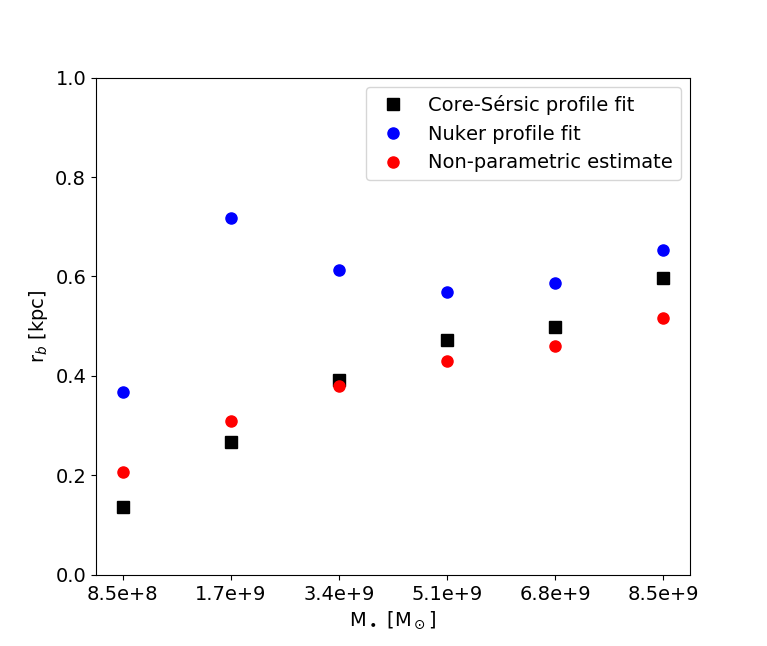
\includegraphics[width=0.7\textwidth]{rb_mass_relation.png}
	\caption{Comparison of core radii of the merger remnants, gained through three different methods; Core-Sérsic profile fitting (black squares), Nuker profile fitting (blue circles) and using equation (tähän kaava!) for finding the "cusp radius" (red circles).}
\end{figure}

\section{Kinematic Properties}

\begin{figure}[h]
	\centering
	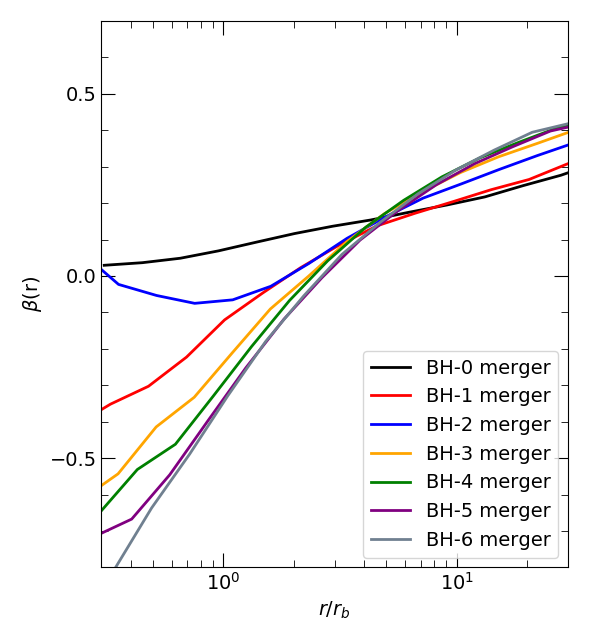
\includegraphics[width=0.9\textwidth]{beta.png}
	\caption{Velocity anisotropy (beta) profiles of the simulated merger remnants with central black holes.}
\end{figure}

\section{Comparison to Observations}

\begin{figure}[h]
	\centering
	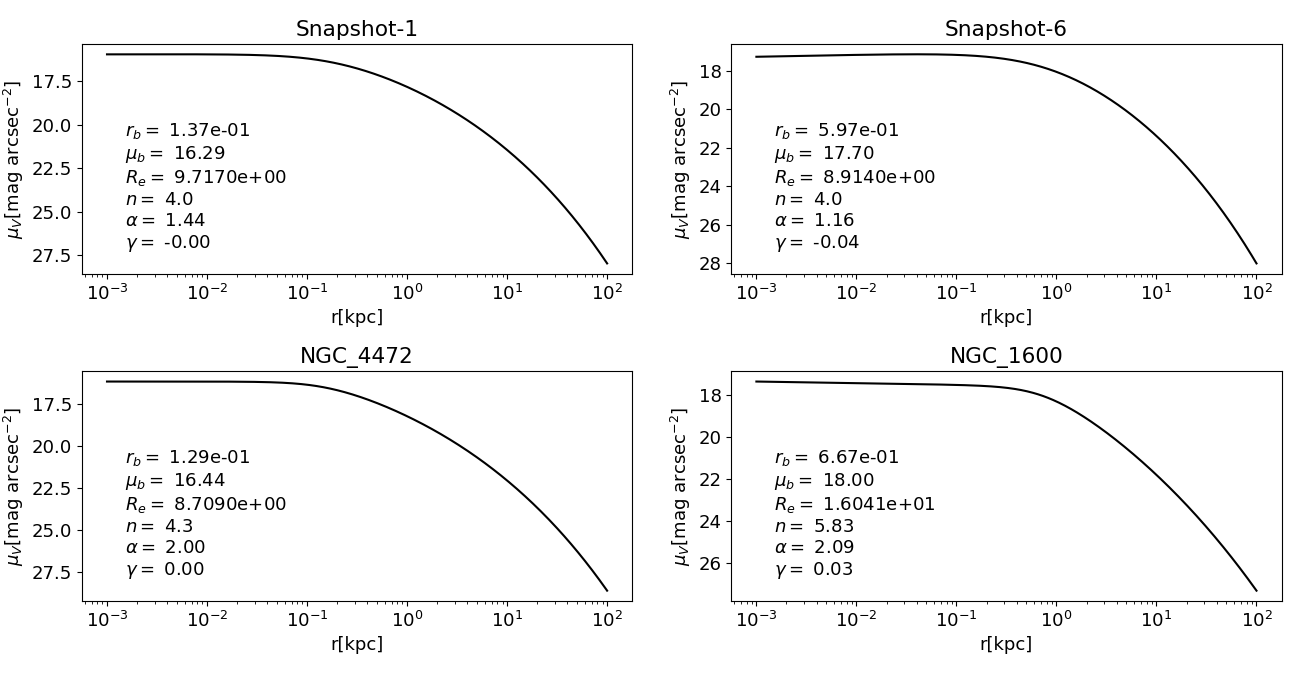
\includegraphics[width=\textwidth]{core_sersic_fits_obs_and_sim.png}
	\caption{Core-Sérsic profile fits of surface brightness profiles calculated from either merger simulation results (top figures) or observed galaxies (bottom figures). The respective fit parameters are written on the figures in units that correspond to the axes. The progenitors of the top-left simulation contained $8.5 \times 10^8 M_\odot$ mass central SMBHs, and $8.5 \times 10^9 M_\odot$ mass central SMBHs in the top-right simulation. The parameters for NGC1600's profile (bottom right), are changed from the units used by \cite{Thomas2016} to the above by assuming $V - R = 0.5$ (the same assumption being done by \cite{Lauer2007}), and by using the distance $D = 64 \mathrm{Mpc}$ \citep{Thomas2016} in order to define the relation between arc seconds and parsecs. As one can see, the profiles gained from simulations and observations are quite similar to each other.}
\end{figure}

\begin{figure}[h]
	\centering
	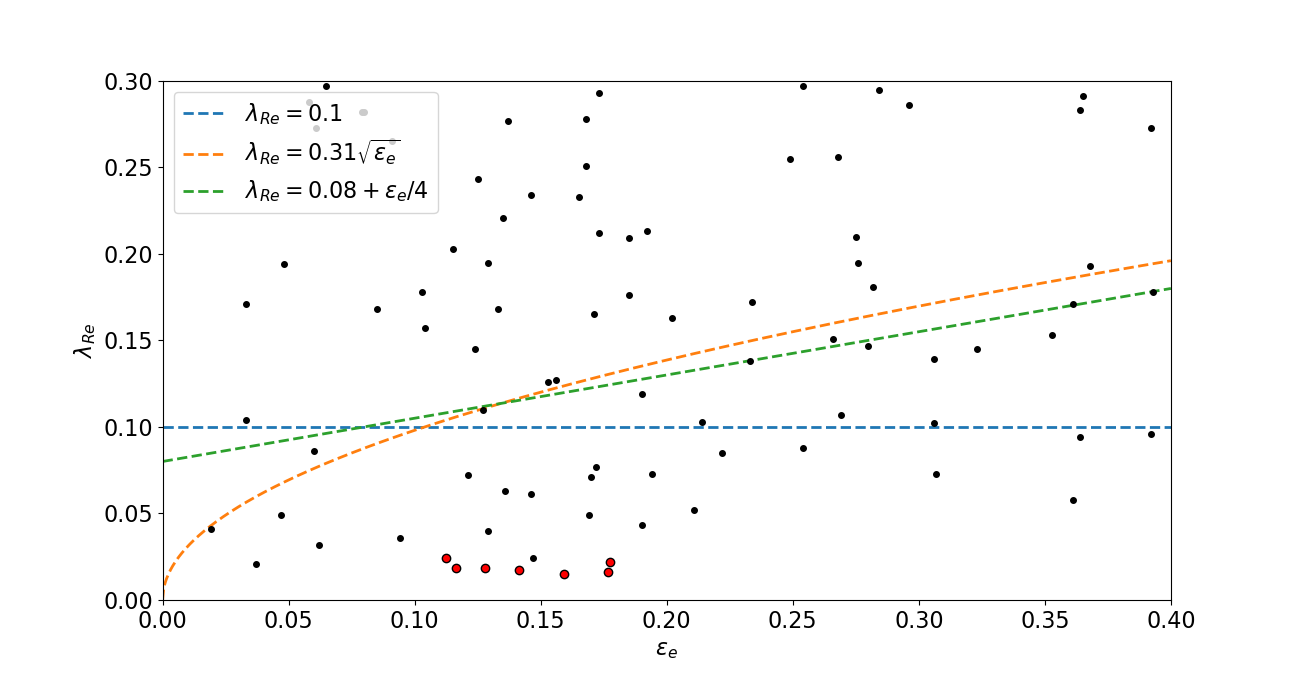
\includegraphics[width=\textwidth]{lambda_epsilon.png}
	\caption{The values of the $\lambda_{\mathrm{Re}}$-parameter of galaxies, plotted against their ellipticity at the effective radius. The red dots correspond to the simulated merger remnants, where as the black dots correspond to galaxies observed in the $\mathrm{ATLAS^{3D}}$-survey \citep{Emsellem2011}. The dashed lines display different slow rotator thresholds as a function of ellipticity.}
\end{figure}

\begin{figure}
	\centering
	\begin{subfigure}[b]{0.49\textwidth}
		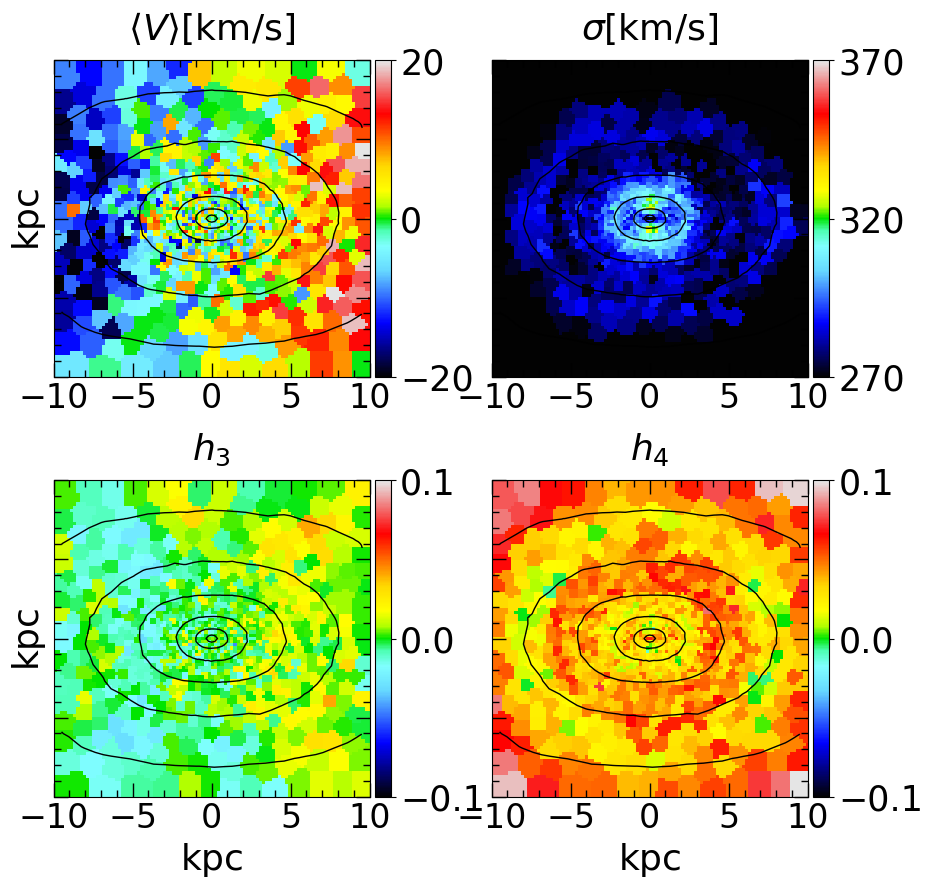
\includegraphics[width=\textwidth]{BH_0.png}
		\caption{BH-0}
	\end{subfigure}
	\begin{subfigure}[b]{0.49\textwidth}
		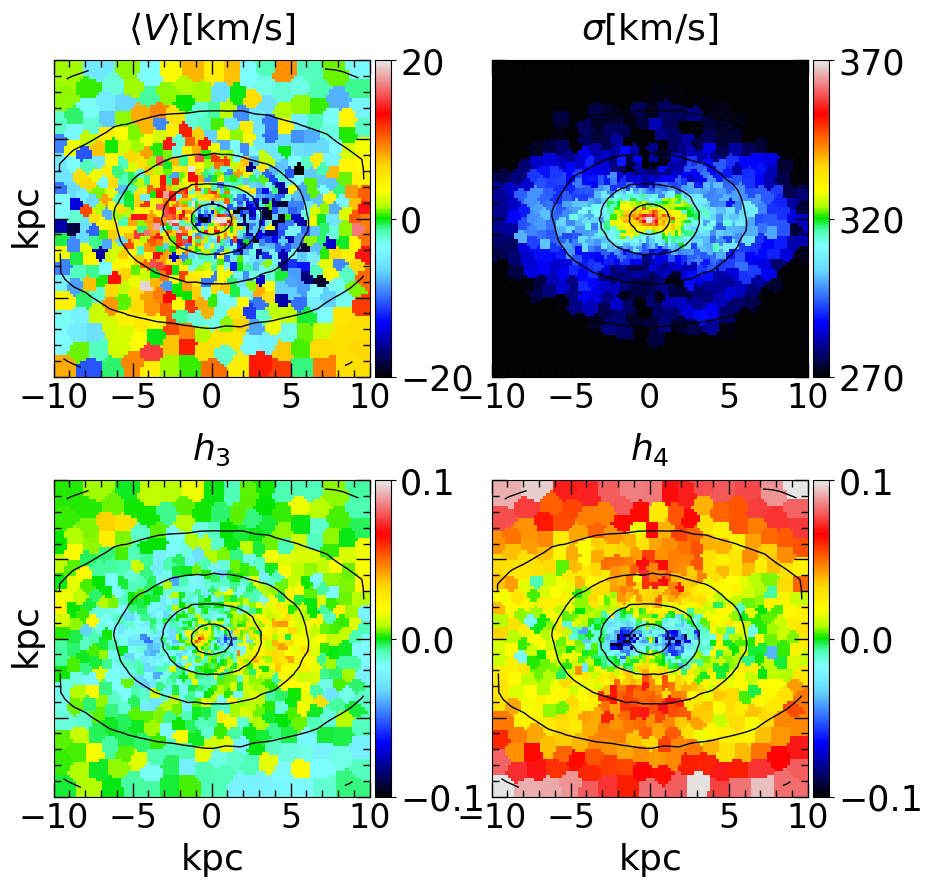
\includegraphics[width=\textwidth]{BH_6.png}
		\caption{BH-6}
	\end{subfigure}
	\caption{IFU-maps of average LOS-velocities, velocity dispersion, $h_3$ parameters and $h_4$ parameters from two simulated merger remnants. The four maps on the left are from a merger simulation where the progenitor galaxies had no central SMBHs, where as the four on the right are from a simulation with progenitor galaxies containing $M_\bullet = 8.5 \times 10^9 M_\odot$ central black holes.}
\end{figure}

\begin{figure}
	\centering
	\begin{subfigure}[b]{0.49\textwidth}
		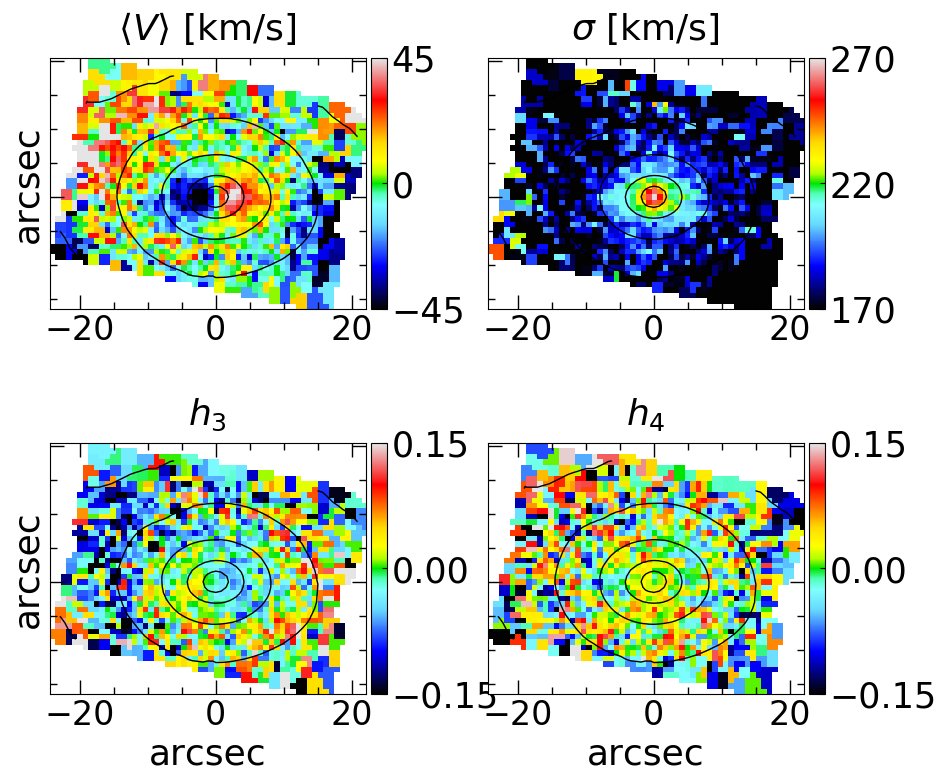
\includegraphics[width=\textwidth]{NGC3414_r6_voronoi.png}
		\caption{NGC 3414}
	\end{subfigure}
	\begin{subfigure}[b]{0.49\textwidth}
		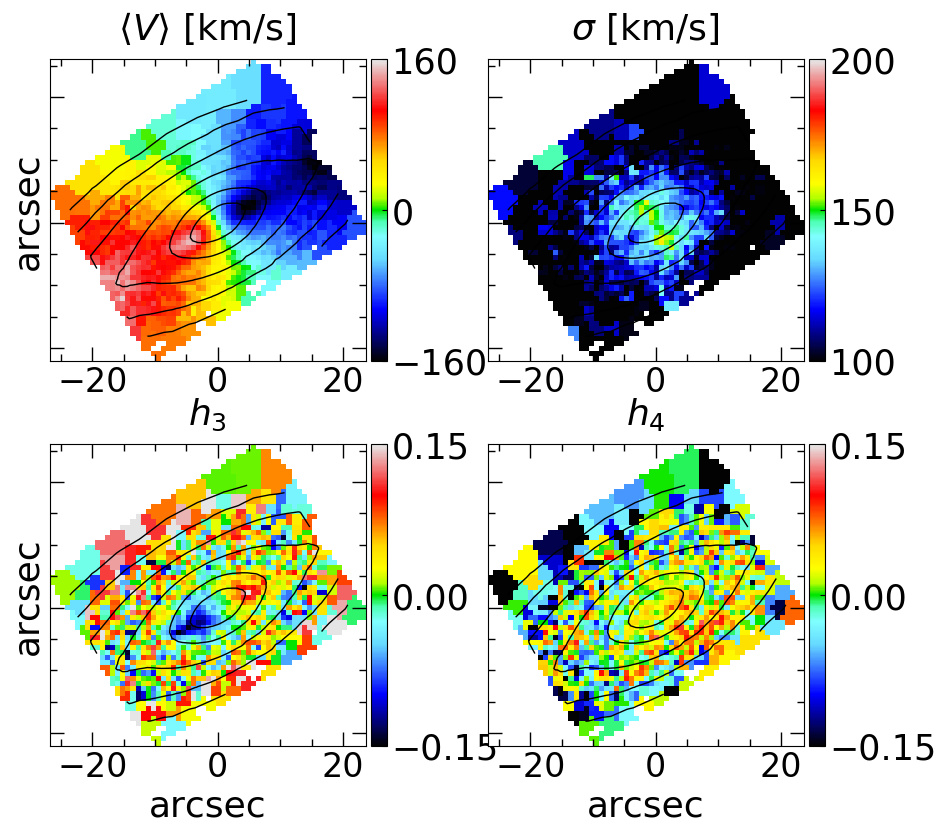
\includegraphics[width=\textwidth]{NGC4111_r1_voronoi.png}
		\caption{NGC 4111}
	\end{subfigure}
	\caption{IFU-maps of average LOS-velocities, velocity dispersion, $h_3$ parameters and $h_4$ parameters from ATLAS3D observations of two galaxies (NGC 3414 \citep{Emsellem2004} and NGC 4111 \citep{Cappellari2011}).}
\end{figure}

\begin{table}
	\begin{center}
		\scriptsize
		\begin{tabular}{c c c c c c c c c c}
		\hline
		\hline
		Galaxy & $M_\star$ & $M_\bullet$ & $R_e$ & $\mu_e$ & $n$ & 
		$\langle V_\mathrm{LOS} \rangle$ & $\sigma_e$ & $\lambda_e$ &
		$\epsilon_e$ \\
		& $[\times 10^{11} M_\odot]$ & $[\times 10^{10} M_\odot]$ &
		[kpc] & [$\mathrm{mag/arcsec^2}$] & & [km/s] & [km/s] & & \\
		(1) & (2) & (3) & (4) & (5) & (6) & (7) & (8) & (9) & (10) \\
		\hline
		BH-6 & $4.960$ & $2 \times 0.85$ & $5.507$ & $20.26$ & $4$ & $6.9$ & $311$ & $0.024$ & $0.11$ \\
		NGC 1600 & $5.0$ & $1.7$ & $\sim 16$ & $(22.53)$ & $5.83$ & $3.4$ & 
		$293$ & $0.026$ & $032$ \\
		\hline
		\end{tabular}
	\end{center}
	\caption{Comparison between the physical properties of the simulated merger remnant "BH-6" and the galaxy NGC 1600. The properties described in the columns of the table are explained below, with the sources for the properties of NGC 1600 being written inside the brackets. \\
	(1) Name of the galaxy. \\
	(2) Total stellar mass \citep{Thomas2016}. \\
	(3) Central black hole mass \citep{Thomas2016}. \\
	(4) Effective radius \citep{Thomas2016}. For NGC 1600, the effective radius is changed from arc seconds to kpc by assuming that it is located at the distance of $D = 64 \; \mathrm{Mpc}$ \citep{Thomas2016}. \\
	(5) Surface brightness at the effective radius. \\
	(6) Sérsic index from the best fitting core-Sérsic profile fit \citep{Thomas2016}. \\
	(7) Mean line-of-sight velocity inside the effective radius \citep{Bender1994}. \\
	(8) Velocity dispersion inside the effective radius \citep{Veale2017veldisp}. For "BH-6", the given velocity dispersion is calculated from a Voronoi binned image as the mean of the velocity dispersion values of the bins located inside the effective radius. \\
	(9) Spin parameter at the effective radius \citep{Veale2018lambda}. \\
	(10) For "BH-6": ellipticity of the galaxy at the effective radius; and for GC 1600: luminosity weighted ellipticity \citep{Goullaud2018}.
	}
\end{table}


\section{Implications}


\chapter{Conclusions}

% STEP 5:
% Uncomment the following lines and set your .bib file and desired bibliography style
% to make a bibliography with BibTeX.
% Alternatively you can use the thebibliography environment if you want to add all
% references by hand.


% Define journal names
\newcommand{\apj}{The Astrophysical Journal}
\newcommand{\mnras}{Monthly Notices of the Royal Astronomical Society}
\newcommand{\apjs}{The Astrophysical Journal Supplement}
\newcommand{\nat}{Nature}
\newcommand{\aj}{The Astronomical Journal}

\clearpage
\addcontentsline{toc}{chapter}{Bibliography} % This lines adds the bibliography to the ToC
\bibliographystyle{plainnat}
\bibliography{bibliography.bib}


\end{document}

